\section{模型求解与结果分析}

\subsection{评价范围与结果来源}

问题一使用附件1的单日数据。其余四组正式结果均覆盖2025年2月1日至12月31日334天，每天144段。所有同一问题的对照使用共同的2月初态，状态逐日连续，不在每天零时重置。由于四问信息和价格环境不同，各自一月运行形成的期初库存分别列示。主案冻结为28场景、无额外CVaR及备用、规则执行，回测期不根据某个消融结果重新改选主案。

表\ref{tab:annual_summary}由实际执行数组汇总。总费用等于计划、调整及紧急费用之和，不含辅助终端项；日总费用CVaR95为334个日账单上5\%尾部的经验风险指标。指定时段购电量及全天常规量不含紧急量，紧急量另列，指定日期的全天费用包含全部实际收费。附件5计划页保留计划费用，调整页填写最终生效量及全部实际费用；无调整页的情形可通过逐日汇总CSV核对完整账单。

\begin{table}[htbp]\centering\small
\caption{最终分问配置的334天开发期闭环评价结果}
\label{tab:annual_summary}
\begin{tabularx}{\linewidth}{LRRRR}\toprule
指标 & 问题2 & 问题3 & 问题4日前版 & 问题4滚动版\\\midrule
计划费用/万元 & 1350.80 & 1350.31 & 1428.01 & 1426.52\\
调整费用/万元 & 0.00 & 24.87 & 0.00 & 28.31\\
紧急费用/万元 & 50.48 & 11.97 & 51.40 & 12.19\\
实际总费用/万元 & 1401.28 & 1387.15 & 1479.41 & 1467.02\\
紧急电量/kWh & 85017.69 & 21029.90 & 80544.00 & 21293.41\\
紧急购电天数 & 113 & 119 & 106 & 116\\
紧急购电连续时段数 & 205 & 204 & 195 & 193\\
日总费用CVaR95/元 & 70731.74 & 65552.76 & 83044.31 & 77575.87\\
最高日费用/元 & 89306.82 & 67941.61 & 108080.37 & 81797.18\\
2月1日期初库存/kWh & 8875.19 & 8814.60 & 9251.54 & 9030.40\\
12月31日期末库存/kWh & 6240.32 & 6240.32 & 6269.86 & 6274.99\\
\bottomrule\end{tabularx}
\par\smallskip\parbox{\linewidth}{\footnotesize 问题2与问题4日前版沿用母模型；问题3与问题4滚动版在零时及日内均启用候选筛选。预测器与实时执行器沿用原冻结配置，筛选适用问题与时点依据开发期比较确定。实际费用不含候选评分的终端偏离项；CVaR95为实际日总账单的经验尾部均值。}
\end{table}


\subsection{问题一：确定性调度结果}

问题一计划购电量为59482.6990 kWh，购电费用35126.9486元。无储能基准按每段$[L_t-R_t]_+\Delta t$购电，费用48052.05元，故节省12925.10元，节费率26.90\%。电池外侧累计充电20740.67 kWh、放电16799.94 kWh，满足$0.9\sum_tc_t=\sum_td_t/0.9$，首末储电量均为6000 kWh。问题一数值在既定时间与两侧效率解释下保持不变。

图\ref{fig:q1}显示低价购电与光伏富余共同承担补能，高价段用储能降低外购需求。储能并非每遇负荷即放空，计划同时考虑后续补能机会、容量与日末回补。题目没有给出爬坡或启停限制，故不对原始最优解作额外平滑。此结果将给定数据视为确定输入，不能直接用来声称未知实际负荷条件下的完美预测优势。

\begin{table}[htbp]\centering\small\caption{问题1指定时段与全天购电结果（电量单位：kWh）}\label{tab:q1-purchase}\begin{tabularx}{\linewidth}{lRlRlR}
\toprule
时间段 & 购电量 & 时间段 & 购电量 & 时间段 & 购电量\\
\midrule
10:00--10:10 & 0.00 & 12:00--12:10 & 480.41 & 14:00--14:10 & 0.00\\
16:00--16:10 & 445.43 & 18:00--18:10 & 531.89 & 20:00--20:10 & 0.00\\
\midrule
全天购电量 & 59482.70 & \multicolumn{2}{c}{全天购电费（元）} & \multicolumn{2}{r}{35126.95}\\
\bottomrule
\end{tabularx}\end{table}
\begin{table}[htbp]\centering\small\caption{问题1储能充放电及首末电量（单位：kWh）}\label{tab:q1-battery}\begin{tabularx}{\linewidth}{lRRlRR}
\toprule
时间段 & 充电量 & 放电量 & 时间段 & 充电量 & 放电量\\
\midrule
00:00--04:00 & 4500.00 & 0.00 & 04:00--08:00 & 833.33 & 6365.84\\
08:00--12:00 & 4787.96 & 1703.00 & 12:00--16:00 & 5286.04 & 91.10\\
16:00--20:00 & 0.00 & 5780.13 & 20:00--24:00 & 5333.33 & 2859.87\\
\midrule
0:00储电量 & \multicolumn{2}{r}{6000.00} & 24:00储电量 & \multicolumn{2}{r}{6000.00}\\
\bottomrule
\end{tabularx}\end{table}
\begin{figure}[htbp]\centering
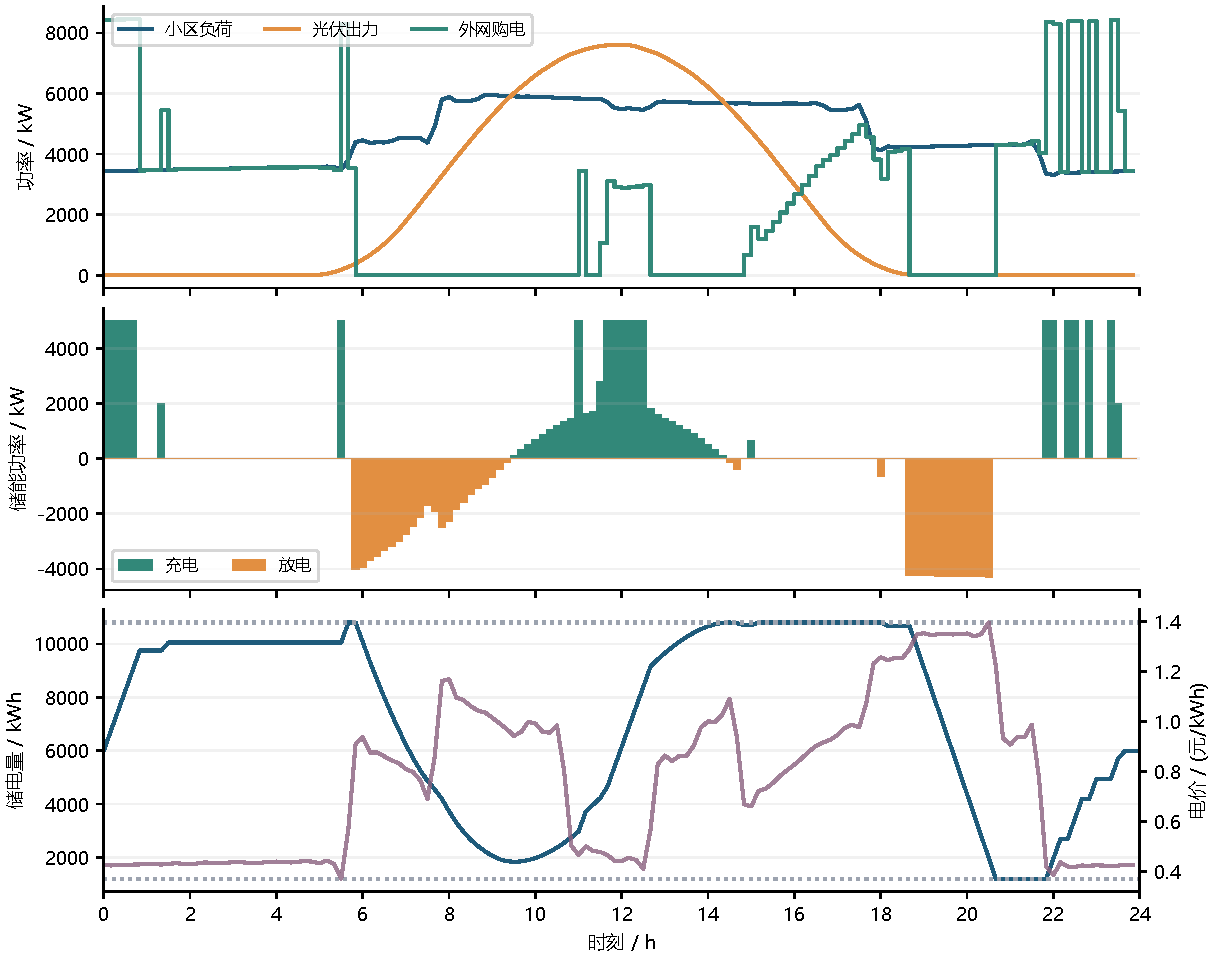
\includegraphics[width=0.94\linewidth]{figures/results/q1_dispatch.pdf}
\caption{问题一购电、充放电、储电量及电价}\label{fig:q1}
\end{figure}
\FloatBarrier

\subsection{问题二：场景采购的经济贡献}

评价期计划费用13507968.43元、紧急费用504839.24元，总费用14012807.66元，紧急购电85017.69 kWh，涉及113天、617个10分钟时段。紧急补购后逐段满足负载；出现紧急购电表示额外昂贵采购，不表示已经发生失供电。

表\ref{tab:v2_baselines}固定同一预测器、执行器及评价期初态。点预测采购费用15290840.75元，无储能场景采购费用18548033.07元。相较点预测，场景期望费用方案节省1278033.08元，即8.36\%；相较无储能场景采购节省24.45\%。主要收益来自对五倍补购的非对称代价进行场景评估，以及电池的跨时段能量转移。该证据支持场景采购，但不意味着必须额外加入风险惩罚。

\begin{table}[htbp]\centering\small
\caption{问题2在相同预测与初态下的基础对照}
\label{tab:v2_baselines}
\begin{tabularx}{\linewidth}{LRRRR}\toprule
策略 & 总费/万元 & 紧急量/kWh & 日费CVaR95/元 & 末库存/kWh\\\midrule
无储能场景采购 & 1854.80 & 242340.86 & 80425.37 & 8875.19\\
点预测采购 & 1529.08 & 505585.75 & 100557.90 & 5845.40\\
场景期望费用（主案） & 1401.28 & 85017.69 & 70731.74 & 6240.32\\
\bottomrule\end{tabularx}
\par\smallskip\parbox{\linewidth}{\footnotesize 本表基于未启用候选筛选的母模型，各组保留原实验配置及数值，覆盖相同334天并连续推进状态；不作为最终筛选算法的同条件消融。}
\end{table}

\begin{table}[htbp]\centering\small
\caption{问题2指定日期购电结果（沿用题目表1布局，电量单位：kWh）}
\label{tab:q2-purchase}
\par\smallskip\textbf{2025-03-20}\par\smallskip
\begin{tabularx}{\linewidth}{lRlRlR}
\toprule
时间段 & 购电量 & 时间段 & 购电量 & 时间段 & 购电量\\
\midrule
10:00--10:10 & 0.00 & 12:00--12:10 & 564.20 & 14:00--14:10 & 0.00\\
16:00--16:10 & 490.32 & 18:00--18:10 & 704.86 & 20:00--20:10 & 0.00\\
\midrule
全天购电量 & 67796.64 & \multicolumn{2}{c}{全天购电费（元）} & \multicolumn{2}{r}{41219.41}\\
\bottomrule
\end{tabularx}
\par\smallskip\textbf{2025-06-21}\par\smallskip
\begin{tabularx}{\linewidth}{lRlRlR}
\toprule
时间段 & 购电量 & 时间段 & 购电量 & 时间段 & 购电量\\
\midrule
10:00--10:10 & 0.00 & 12:00--12:10 & 0.00 & 14:00--14:10 & 0.00\\
16:00--16:10 & 296.43 & 18:00--18:10 & 275.52 & 20:00--20:10 & 0.00\\
\midrule
全天购电量 & 40036.30 & \multicolumn{2}{c}{全天购电费（元）} & \multicolumn{2}{r}{23986.38}\\
\bottomrule
\end{tabularx}
\par\smallskip\textbf{2025-09-23}\par\smallskip
\begin{tabularx}{\linewidth}{lRlRlR}
\toprule
时间段 & 购电量 & 时间段 & 购电量 & 时间段 & 购电量\\
\midrule
10:00--10:10 & 0.00 & 12:00--12:10 & 475.29 & 14:00--14:10 & 0.00\\
16:00--16:10 & 537.29 & 18:00--18:10 & 789.93 & 20:00--20:10 & 0.00\\
\midrule
全天购电量 & 69576.50 & \multicolumn{2}{c}{全天购电费（元）} & \multicolumn{2}{r}{46384.26}\\
\bottomrule
\end{tabularx}
\par\smallskip\textbf{2025-12-21}\par\smallskip
\begin{tabularx}{\linewidth}{lRlRlR}
\toprule
时间段 & 购电量 & 时间段 & 购电量 & 时间段 & 购电量\\
\midrule
10:00--10:10 & 0.00 & 12:00--12:10 & 970.92 & 14:00--14:10 & 0.00\\
16:00--16:10 & 851.12 & 18:00--18:10 & 744.23 & 20:00--20:10 & 0.00\\
\midrule
全天购电量 & 101008.53 & \multicolumn{2}{c}{全天购电费（元）} & \multicolumn{2}{r}{65454.44}\\
\bottomrule
\end{tabularx}
\par\smallskip\parbox{\linewidth}{\footnotesize 注：问题2与4-2列示计划购电量；问题3与4-3列示最终生效的调整后常规购电量。全天购电量不含紧急购电，全天购电费含计划、调整与紧急费用。}
\end{table}

\begin{table}[htbp]\centering\small
\caption{问题2指定日期储能结果（沿用题目表2布局，单位：kWh）}
\label{tab:q2-battery}
\par\smallskip\textbf{2025-03-20}\par\smallskip
\begin{tabularx}{\linewidth}{lRRlRR}
\toprule
时间段 & 充电量 & 放电量 & 时间段 & 充电量 & 放电量\\
\midrule
00:00--04:00 & 3924.13 & 181.53 & 04:00--08:00 & 1015.09 & 5240.21\\
08:00--12:00 & 6123.03 & 2777.38 & 12:00--16:00 & 3923.99 & 420.71\\
16:00--20:00 & 268.54 & 5719.49 & 20:00--24:00 & 5703.85 & 2960.43\\
\midrule
0:00储电量 & \multicolumn{2}{r}{6705.54} & 24:00储电量 & \multicolumn{2}{r}{6346.37}\\
\bottomrule
\end{tabularx}
\par\smallskip\textbf{2025-06-21}\par\smallskip
\begin{tabularx}{\linewidth}{lRRlRR}
\toprule
时间段 & 充电量 & 放电量 & 时间段 & 充电量 & 放电量\\
\midrule
00:00--04:00 & 1394.50 & 465.11 & 04:00--08:00 & 460.19 & 4390.39\\
08:00--12:00 & 6534.90 & 0.00 & 12:00--16:00 & 0.00 & 0.00\\
16:00--20:00 & 156.59 & 4882.20 & 20:00--24:00 & 6792.80 & 2485.90\\
\midrule
0:00储电量 & \multicolumn{2}{r}{8644.37} & 24:00储电量 & \multicolumn{2}{r}{8867.68}\\
\bottomrule
\end{tabularx}
\par\smallskip\textbf{2025-09-23}\par\smallskip
\begin{tabularx}{\linewidth}{lRRlRR}
\toprule
时间段 & 充电量 & 放电量 & 时间段 & 充电量 & 放电量\\
\midrule
00:00--04:00 & 4692.99 & 53.14 & 04:00--08:00 & 916.24 & 5893.48\\
08:00--12:00 & 5977.49 & 1896.62 & 12:00--16:00 & 3708.39 & 625.98\\
16:00--20:00 & 151.78 & 5739.35 & 20:00--24:00 & 5609.40 & 2640.89\\
\midrule
0:00储电量 & \multicolumn{2}{r}{6006.02} & 24:00储电量 & \multicolumn{2}{r}{6235.06}\\
\bottomrule
\end{tabularx}
\par\smallskip\textbf{2025-12-21}\par\smallskip
\begin{tabularx}{\linewidth}{lRRlRR}
\toprule
时间段 & 充电量 & 放电量 & 时间段 & 充电量 & 放电量\\
\midrule
00:00--04:00 & 4499.79 & 40.16 & 04:00--08:00 & 762.27 & 1359.20\\
08:00--12:00 & 5913.75 & 6490.57 & 12:00--16:00 & 5645.48 & 2130.65\\
16:00--20:00 & 0.00 & 5526.27 & 20:00--24:00 & 5771.81 & 2842.53\\
\midrule
0:00储电量 & \multicolumn{2}{r}{6794.81} & 24:00储电量 & \multicolumn{2}{r}{6695.97}\\
\bottomrule
\end{tabularx}
\end{table}

\begin{table}[htbp]\centering\small
\caption{问题2指定日期紧急购电（题目表3布局，单位：kWh）}
\label{tab:q2-emergency}
\setlength{\tabcolsep}{3pt}
\begin{tabularx}{\linewidth}{lRlRlRlR}\toprule
\multicolumn{2}{c}{2025-03-20} & \multicolumn{2}{c}{2025-06-21} & \multicolumn{2}{c}{2025-09-23} & \multicolumn{2}{c}{2025-12-21}\\
时间段 & 购电量 & 时间段 & 购电量 & 时间段 & 购电量 & 时间段 & 购电量\\\midrule
无 & 0.00 & 无 & 0.00 & 20:20--20:40 & 388.40 & 无 & 0.00\\
 &   &  &   & 20:50--21:10 & 90.05 &  &  \\
 &   &  &   & 21:20--21:50 & 34.20 &  &  \\
\midrule
合计 & 0.00 & 合计 & 0.00 & 合计 & 512.64 & 合计 & 0.00\\
\bottomrule\end{tabularx}\end{table}

四个指定日期中，9月23日存在三段紧急购电，合计512.64 kWh，其余三个日期为零。相邻正值时段才合并，夹有零紧急量时保留分段。四小时区间内充、放电量可以同时为正，表示不同10分钟时段各自充电或放电，不违反单时段互斥。
\FloatBarrier

\subsection{问题三：交易修订与反馈来源}

问题三计划费用13674565.95元、调整费用230664.95元、紧急费用70579.96元，总费用13975810.86元。紧急购电12647.76 kWh，涉及92天、282个时段。与问题二相比，费用降低0.2640\%，紧急量降低85.12\%。两问零时光伏信息不同、各自一月末态也不同，因此这一横向差异不是滚动更新本身的独立因果收益。

为区分信息来源，表\ref{tab:v2_feedback}在同一问题三模型下依次比较：仅零时外层计划；6、12、18时仅更新SOC并按零时预测重优化；再加入新发布光伏；最后加入已观测负荷偏差反馈。四组均采用规则执行，不启用跨日候选，因此不会通过续接预测把新信息带入“SOC-only”组。

\begin{table}[htbp]\centering\small
\caption{问题3母模型的状态、光伏和负荷反馈分解}
\label{tab:v2_feedback}
\begin{tabularx}{\linewidth}{LRRRR}\toprule
策略 & 总费/万元 & 紧急量/kWh & 日费CVaR95/元 & 末库存/kWh\\\midrule
仅零时外层计划 & 1416.90 & 80181.62 & 71801.23 & 6240.32\\
仅更新SOC并重优化 & 1399.17 & 39298.96 & 66748.14 & 6240.32\\
再加入新光伏预报 & 1407.57 & 40071.16 & 66732.97 & 6240.32\\
再加入负荷偏差反馈 & 1397.58 & 12647.76 & 65518.79 & 6240.32\\
\bottomrule\end{tabularx}
\par\smallskip\parbox{\linewidth}{\footnotesize 本表基于未启用候选筛选的母模型，各组保留原实验配置及数值，覆盖相同334天并连续推进状态；不作为最终筛选算法的同条件消融。}
\end{table}


仅零时外层计划的费用为14169011.89元，更新SOC并重优化后降至13991697.93元，减少177313.97元；再加入新光伏预报，费用增至14075665.67元；进一步加入负荷偏差反馈，费用降至13975810.86元。新光伏这一增量在本回测中增加83967.74元，随后负荷反馈减少99854.81元。这些是相同设置下的闭环路径差异，体现采购、状态和预测误差相互作用，不能将每份新预报的价值预设为正。所有预报发布时间以外的新预报均未由附件提供，不能用实际未来光伏代替不存在的高频预报来计算收益。

图\ref{fig:v2-control}选取评价期紧急购电量最大日7月4日，以独立纵轴显示上调量、参考与实际SOC、紧急量。清晨实际电量比参考更早触及下限，6时前集中补购；中午参考轨迹因外层重新初始化出现跳变，不能将拼接参考曲线当成一条连续实施轨迹。图\ref{fig:v2-adjustments}另列四个指定日期的调整量，避免计划与最终购电曲线重合掩盖修订幅度。

\begin{figure}[htbp]\centering
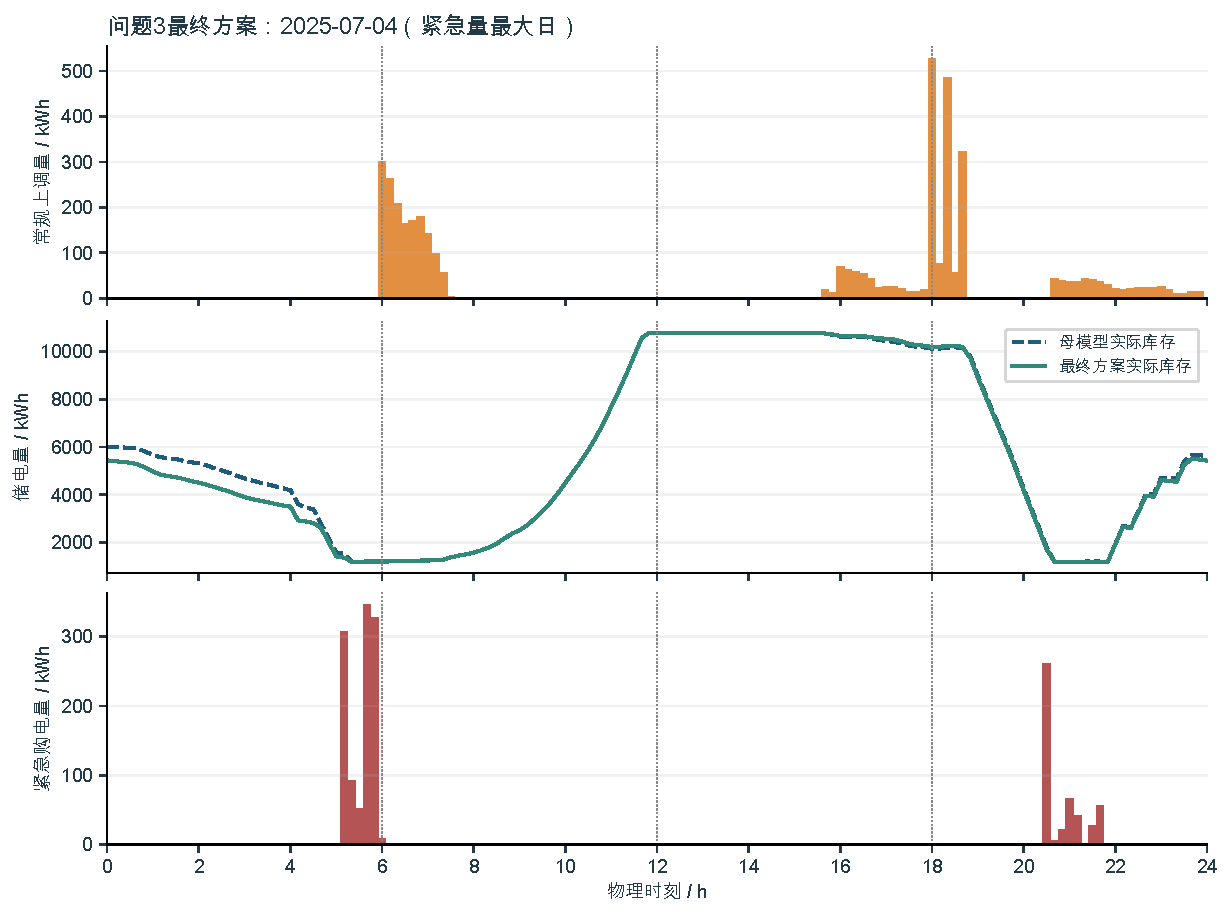
\includegraphics[width=0.96\linewidth]{figures/results/v2_control_difference.pdf}
\caption{问题三紧急量最大日的调整、SOC偏差与紧急购电；虚线标示合法外层修订时点}\label{fig:v2-control}
\end{figure}
\begin{figure}[htbp]\centering
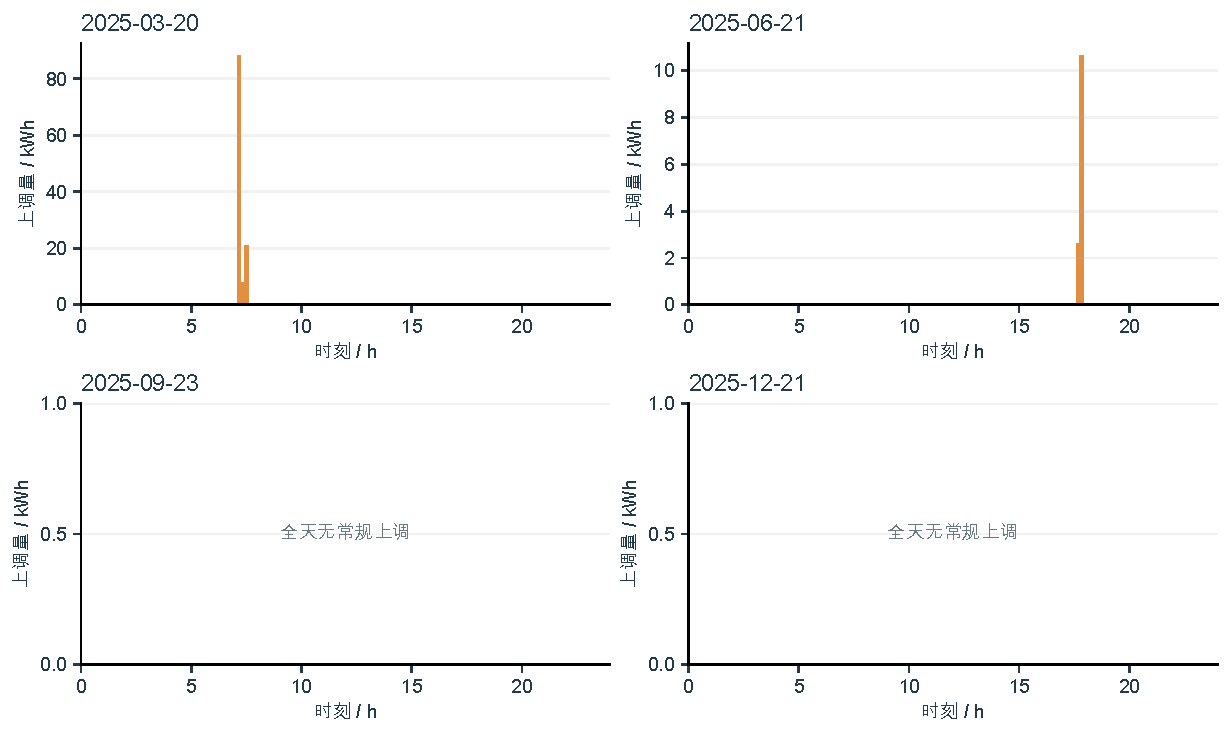
\includegraphics[width=0.96\linewidth]{figures/results/v2_adjustments.pdf}
\caption{四个指定日期的常规购电调整量$a_t-g_t$}\label{fig:v2-adjustments}
\end{figure}
\begin{table}[htbp]\centering\small
\caption{问题3指定日期购电结果（沿用题目表1布局，电量单位：kWh）}
\label{tab:q3-purchase}
\par\smallskip\textbf{2025-03-20}\par\smallskip
\begin{tabularx}{\linewidth}{lRlRlR}
\toprule
时间段 & 购电量 & 时间段 & 购电量 & 时间段 & 购电量\\
\midrule
10:00--10:10 & 0.00 & 12:00--12:10 & 624.29 & 14:00--14:10 & 0.00\\
16:00--16:10 & 671.04 & 18:00--18:10 & 704.20 & 20:00--20:10 & 0.00\\
\midrule
全天购电量 & 71789.01 & \multicolumn{2}{c}{全天购电费（元）} & \multicolumn{2}{r}{45563.84}\\
\bottomrule
\end{tabularx}
\par\smallskip\textbf{2025-06-21}\par\smallskip
\begin{tabularx}{\linewidth}{lRlRlR}
\toprule
时间段 & 购电量 & 时间段 & 购电量 & 时间段 & 购电量\\
\midrule
10:00--10:10 & 0.00 & 12:00--12:10 & 0.00 & 14:00--14:10 & 0.00\\
16:00--16:10 & 260.52 & 18:00--18:10 & 0.00 & 20:00--20:10 & 0.00\\
\midrule
全天购电量 & 37273.13 & \multicolumn{2}{c}{全天购电费（元）} & \multicolumn{2}{r}{21986.55}\\
\bottomrule
\end{tabularx}
\par\smallskip\textbf{2025-09-23}\par\smallskip
\begin{tabularx}{\linewidth}{lRlRlR}
\toprule
时间段 & 购电量 & 时间段 & 购电量 & 时间段 & 购电量\\
\midrule
10:00--10:10 & 0.00 & 12:00--12:10 & 444.81 & 14:00--14:10 & 0.00\\
16:00--16:10 & 611.01 & 18:00--18:10 & 801.37 & 20:00--20:10 & 0.00\\
\midrule
全天购电量 & 73472.67 & \multicolumn{2}{c}{全天购电费（元）} & \multicolumn{2}{r}{46201.57}\\
\bottomrule
\end{tabularx}
\par\smallskip\textbf{2025-12-21}\par\smallskip
\begin{tabularx}{\linewidth}{lRlRlR}
\toprule
时间段 & 购电量 & 时间段 & 购电量 & 时间段 & 购电量\\
\midrule
10:00--10:10 & 0.00 & 12:00--12:10 & 1054.19 & 14:00--14:10 & 0.00\\
16:00--16:10 & 877.48 & 18:00--18:10 & 744.23 & 20:00--20:10 & 0.00\\
\midrule
全天购电量 & 101747.42 & \multicolumn{2}{c}{全天购电费（元）} & \multicolumn{2}{r}{65702.81}\\
\bottomrule
\end{tabularx}
\par\smallskip\parbox{\linewidth}{\footnotesize 注：问题2与4-2列示计划购电量；问题3与4-3列示最终生效的调整后常规购电量。全天购电量不含紧急购电，全天购电费含计划、调整与紧急费用。}
\end{table}

\begin{table}[htbp]\centering\small
\caption{问题3指定日期储能结果（沿用题目表2布局，单位：kWh）}
\label{tab:q3-battery}
\par\smallskip\textbf{2025-03-20}\par\smallskip
\begin{tabularx}{\linewidth}{lRRlRR}
\toprule
时间段 & 充电量 & 放电量 & 时间段 & 充电量 & 放电量\\
\midrule
00:00--04:00 & 4146.19 & 181.53 & 04:00--08:00 & 883.67 & 6201.85\\
08:00--12:00 & 5765.88 & 2465.92 & 12:00--16:00 & 5215.25 & 254.72\\
16:00--20:00 & 1.31 & 5594.70 & 20:00--24:00 & 5703.85 & 2960.43\\
\midrule
0:00储电量 & \multicolumn{2}{r}{6505.69} & 24:00储电量 & \multicolumn{2}{r}{6428.95}\\
\bottomrule
\end{tabularx}
\par\smallskip\textbf{2025-06-21}\par\smallskip
\begin{tabularx}{\linewidth}{lRRlRR}
\toprule
时间段 & 充电量 & 放电量 & 时间段 & 充电量 & 放电量\\
\midrule
00:00--04:00 & 915.21 & 972.82 & 04:00--08:00 & 511.20 & 4390.39\\
08:00--12:00 & 8439.30 & 0.00 & 12:00--16:00 & 0.00 & 0.00\\
16:00--20:00 & 241.25 & 5157.72 & 20:00--24:00 & 6354.48 & 2485.90\\
\midrule
0:00储电量 & \multicolumn{2}{r}{7879.99} & 24:00储电量 & \multicolumn{2}{r}{8243.25}\\
\bottomrule
\end{tabularx}
\par\smallskip\textbf{2025-09-23}\par\smallskip
\begin{tabularx}{\linewidth}{lRRlRR}
\toprule
时间段 & 充电量 & 放电量 & 时间段 & 充电量 & 放电量\\
\midrule
00:00--04:00 & 4692.99 & 53.14 & 04:00--08:00 & 892.10 & 5612.58\\
08:00--12:00 & 6293.08 & 1896.62 & 12:00--16:00 & 3282.98 & 403.62\\
16:00--20:00 & 15.07 & 5619.05 & 20:00--24:00 & 5609.40 & 3045.21\\
\midrule
0:00储电量 & \multicolumn{2}{r}{6006.02} & 24:00储电量 & \multicolumn{2}{r}{6235.06}\\
\bottomrule
\end{tabularx}
\par\smallskip\textbf{2025-12-21}\par\smallskip
\begin{tabularx}{\linewidth}{lRRlRR}
\toprule
时间段 & 充电量 & 放电量 & 时间段 & 充电量 & 放电量\\
\midrule
00:00--04:00 & 4496.41 & 40.16 & 04:00--08:00 & 762.28 & 1406.28\\
08:00--12:00 & 6441.76 & 6526.43 & 12:00--16:00 & 5333.82 & 2222.97\\
16:00--20:00 & 0.00 & 5526.27 & 20:00--24:00 & 5771.81 & 2842.53\\
\midrule
0:00储电量 & \multicolumn{2}{r}{6797.85} & 24:00储电量 & \multicolumn{2}{r}{6695.97}\\
\bottomrule
\end{tabularx}
\end{table}

\begin{table}[htbp]\centering\small
\caption{问题3指定日期紧急购电（题目表3布局，单位：kWh）}
\label{tab:q3-emergency}
\setlength{\tabcolsep}{3pt}
\begin{tabularx}{\linewidth}{lRlRlRlR}\toprule
\multicolumn{2}{c}{2025-03-20} & \multicolumn{2}{c}{2025-06-21} & \multicolumn{2}{c}{2025-09-23} & \multicolumn{2}{c}{2025-12-21}\\
时间段 & 购电量 & 时间段 & 购电量 & 时间段 & 购电量 & 时间段 & 购电量\\\midrule
09:10--10:00 & 311.46 & 无 & 0.00 & 20:20--20:30 & 6.38 & 无 & 0.00\\
 &   &  &   & 20:50--21:10 & 67.74 &  &  \\
 &   &  &   & 21:20--21:50 & 34.20 &  &  \\
\midrule
合计 & 311.46 & 合计 & 0.00 & 合计 & 108.31 & 合计 & 0.00\\
\bottomrule\end{tabularx}\end{table}
\FloatBarrier

\subsection{问题四：联合价格不确定下的采购与滚动调度}

动态电价下静态方案计划费用14280142.03元、紧急费用513982.26元，总费用14794124.29元，紧急电量80544.00 kWh。滚动方案计划费用14460229.83元、调整费用241942.19元、紧急费用67060.51元，总费用14769232.53元，紧急电量11950.68 kWh。两案费用相差24891.76元，即0.1683\%，而紧急电量降低85.16\%。

这一结果说明昂贵补购减少并不必然带来同比例的总费用下降：增加常规承诺和修订仍须付款。滚动案实际日费用CVaR95为77420.84元，静态案为83044.31元；它们是已实现账单的描述，不是风险扩展效果的证明。本节两案的预测配置和期初库存也有所区别，费用差不能全部归为单个价格预测或控制模块。

联合场景采用同日价荷残差，依据价格加权分位数的机制解释，高缺口是否伴随高电价会影响采购。有限历史窗口并不能覆盖所有价荷状态，不能把单时段80\%分位数直接用作含储能系统的逐时公式。四个指定日期的常规采购、储能与紧急结果如下，具体计划费与调整费分解附于支撑表。

\begin{table}[htbp]\centering\small
\caption{问题4-2指定日期购电结果（沿用题目表1布局，电量单位：kWh）}
\label{tab:q4_2-purchase}
\par\smallskip\textbf{2025-03-20}\par\smallskip
\begin{tabularx}{\linewidth}{lRlRlR}
\toprule
时间段 & 购电量 & 时间段 & 购电量 & 时间段 & 购电量\\
\midrule
10:00--10:10 & 0.00 & 12:00--12:10 & 564.20 & 14:00--14:10 & 0.00\\
16:00--16:10 & 490.32 & 18:00--18:10 & 0.00 & 20:00--20:10 & 743.27\\
\midrule
全天购电量 & 67869.67 & \multicolumn{2}{c}{全天购电费（元）} & \multicolumn{2}{r}{42207.16}\\
\bottomrule
\end{tabularx}
\par\smallskip\textbf{2025-06-21}\par\smallskip
\begin{tabularx}{\linewidth}{lRlRlR}
\toprule
时间段 & 购电量 & 时间段 & 购电量 & 时间段 & 购电量\\
\midrule
10:00--10:10 & 0.00 & 12:00--12:10 & 0.00 & 14:00--14:10 & 0.00\\
16:00--16:10 & 296.43 & 18:00--18:10 & 510.07 & 20:00--20:10 & 0.00\\
\midrule
全天购电量 & 40675.72 & \multicolumn{2}{c}{全天购电费（元）} & \multicolumn{2}{r}{21012.94}\\
\bottomrule
\end{tabularx}
\par\smallskip\textbf{2025-09-23}\par\smallskip
\begin{tabularx}{\linewidth}{lRlRlR}
\toprule
时间段 & 购电量 & 时间段 & 购电量 & 时间段 & 购电量\\
\midrule
10:00--10:10 & 0.00 & 12:00--12:10 & 497.24 & 14:00--14:10 & 0.00\\
16:00--16:10 & 537.29 & 18:00--18:10 & 0.00 & 20:00--20:10 & 0.00\\
\midrule
全天购电量 & 69762.68 & \multicolumn{2}{c}{全天购电费（元）} & \multicolumn{2}{r}{48309.88}\\
\bottomrule
\end{tabularx}
\par\smallskip\textbf{2025-12-21}\par\smallskip
\begin{tabularx}{\linewidth}{lRlRlR}
\toprule
时间段 & 购电量 & 时间段 & 购电量 & 时间段 & 购电量\\
\midrule
10:00--10:10 & 0.00 & 12:00--12:10 & 970.92 & 14:00--14:10 & 0.00\\
16:00--16:10 & 851.12 & 18:00--18:10 & 744.23 & 20:00--20:10 & 0.00\\
\midrule
全天购电量 & 100945.95 & \multicolumn{2}{c}{全天购电费（元）} & \multicolumn{2}{r}{77020.40}\\
\bottomrule
\end{tabularx}
\par\smallskip\parbox{\linewidth}{\footnotesize 注：问题2与4-2列示计划购电量；问题3与4-3列示最终生效的调整后常规购电量。全天购电量不含紧急购电，全天购电费含计划、调整与紧急费用。}
\end{table}

\begin{table}[htbp]\centering\small
\caption{问题4-2指定日期储能结果（沿用题目表2布局，单位：kWh）}
\label{tab:q4_2-battery}
\par\smallskip\textbf{2025-03-20}\par\smallskip
\begin{tabularx}{\linewidth}{lRRlRR}
\toprule
时间段 & 充电量 & 放电量 & 时间段 & 充电量 & 放电量\\
\midrule
00:00--04:00 & 3824.42 & 134.84 & 04:00--08:00 & 1669.83 & 5857.47\\
08:00--12:00 & 6146.04 & 2777.38 & 12:00--16:00 & 3907.13 & 420.71\\
16:00--20:00 & 174.78 & 6369.00 & 20:00--24:00 & 5798.62 & 2212.03\\
\midrule
0:00储电量 & \multicolumn{2}{r}{6834.43} & 24:00储电量 & \multicolumn{2}{r}{6457.15}\\
\bottomrule
\end{tabularx}
\par\smallskip\textbf{2025-06-21}\par\smallskip
\begin{tabularx}{\linewidth}{lRRlRR}
\toprule
时间段 & 充电量 & 放电量 & 时间段 & 充电量 & 放电量\\
\midrule
00:00--04:00 & 963.51 & 3780.66 & 04:00--08:00 & 1400.69 & 1719.95\\
08:00--12:00 & 6932.04 & 0.00 & 12:00--16:00 & 0.00 & 0.00\\
16:00--20:00 & 0.00 & 4853.45 & 20:00--24:00 & 7501.98 & 3091.92\\
\midrule
0:00储电量 & \multicolumn{2}{r}{8545.17} & 24:00储电量 & \multicolumn{2}{r}{8723.59}\\
\bottomrule
\end{tabularx}
\par\smallskip\textbf{2025-09-23}\par\smallskip
\begin{tabularx}{\linewidth}{lRRlRR}
\toprule
时间段 & 充电量 & 放电量 & 时间段 & 充电量 & 放电量\\
\midrule
00:00--04:00 & 5330.27 & 22.20 & 04:00--08:00 & 206.94 & 5820.07\\
08:00--12:00 & 5946.19 & 1896.62 & 12:00--16:00 & 3587.87 & 530.87\\
16:00--20:00 & 163.52 & 6562.31 & 20:00--24:00 & 5525.15 & 1842.66\\
\midrule
0:00储电量 & \multicolumn{2}{r}{6002.76} & 24:00储电量 & \multicolumn{2}{r}{6159.23}\\
\bottomrule
\end{tabularx}
\par\smallskip\textbf{2025-12-21}\par\smallskip
\begin{tabularx}{\linewidth}{lRRlRR}
\toprule
时间段 & 充电量 & 放电量 & 时间段 & 充电量 & 放电量\\
\midrule
00:00--04:00 & 4499.29 & 40.16 & 04:00--08:00 & 0.00 & 741.76\\
08:00--12:00 & 5940.70 & 6486.91 & 12:00--16:00 & 5724.46 & 2220.11\\
16:00--20:00 & 0.00 & 5500.96 & 20:00--24:00 & 5818.48 & 2842.53\\
\midrule
0:00储电量 & \multicolumn{2}{r}{6795.26} & 24:00储电量 & \multicolumn{2}{r}{6766.10}\\
\bottomrule
\end{tabularx}
\end{table}

\begin{table}[htbp]\centering\small
\caption{问题4-2指定日期紧急购电（题目表3布局，单位：kWh）}
\label{tab:q4_2-emergency}
\setlength{\tabcolsep}{3pt}
\begin{tabularx}{\linewidth}{lRlRlRlR}\toprule
\multicolumn{2}{c}{2025-03-20} & \multicolumn{2}{c}{2025-06-21} & \multicolumn{2}{c}{2025-09-23} & \multicolumn{2}{c}{2025-12-21}\\
时间段 & 购电量 & 时间段 & 购电量 & 时间段 & 购电量 & 时间段 & 购电量\\\midrule
无 & 0.00 & 无 & 0.00 & 18:20--18:40 & 3.91 & 无 & 0.00\\
 &   &  &   & 20:30--20:40 & 357.19 &  &  \\
 &   &  &   & 20:50--21:10 & 90.05 &  &  \\
 &   &  &   & 21:20--21:50 & 34.20 &  &  \\
\midrule
合计 & 0.00 & 合计 & 0.00 & 合计 & 485.35 & 合计 & 0.00\\
\bottomrule\end{tabularx}\end{table}
\FloatBarrier
\begin{table}[htbp]\centering\small
\caption{问题4-3指定日期购电结果（沿用题目表1布局，电量单位：kWh）}
\label{tab:q4_3-purchase}
\par\smallskip\textbf{2025-03-20}\par\smallskip
\begin{tabularx}{\linewidth}{lRlRlR}
\toprule
时间段 & 购电量 & 时间段 & 购电量 & 时间段 & 购电量\\
\midrule
10:00--10:10 & 0.00 & 12:00--12:10 & 624.29 & 14:00--14:10 & 0.00\\
16:00--16:10 & 671.04 & 18:00--18:10 & 704.20 & 20:00--20:10 & 743.27\\
\midrule
全天购电量 & 71574.04 & \multicolumn{2}{c}{全天购电费（元）} & \multicolumn{2}{r}{45107.31}\\
\bottomrule
\end{tabularx}
\par\smallskip\textbf{2025-06-21}\par\smallskip
\begin{tabularx}{\linewidth}{lRlRlR}
\toprule
时间段 & 购电量 & 时间段 & 购电量 & 时间段 & 购电量\\
\midrule
10:00--10:10 & 0.00 & 12:00--12:10 & 0.00 & 14:00--14:10 & 0.00\\
16:00--16:10 & 260.52 & 18:00--18:10 & 495.32 & 20:00--20:10 & 0.00\\
\midrule
全天购电量 & 37518.90 & \multicolumn{2}{c}{全天购电费（元）} & \multicolumn{2}{r}{19308.93}\\
\bottomrule
\end{tabularx}
\par\smallskip\textbf{2025-09-23}\par\smallskip
\begin{tabularx}{\linewidth}{lRlRlR}
\toprule
时间段 & 购电量 & 时间段 & 购电量 & 时间段 & 购电量\\
\midrule
10:00--10:10 & 22.75 & 12:00--12:10 & 461.07 & 14:00--14:10 & 54.35\\
16:00--16:10 & 611.01 & 18:00--18:10 & 0.00 & 20:00--20:10 & 822.11\\
\midrule
全天购电量 & 73431.36 & \multicolumn{2}{c}{全天购电费（元）} & \multicolumn{2}{r}{47890.72}\\
\bottomrule
\end{tabularx}
\par\smallskip\textbf{2025-12-21}\par\smallskip
\begin{tabularx}{\linewidth}{lRlRlR}
\toprule
时间段 & 购电量 & 时间段 & 购电量 & 时间段 & 购电量\\
\midrule
10:00--10:10 & 0.00 & 12:00--12:10 & 1054.19 & 14:00--14:10 & 0.00\\
16:00--16:10 & 877.48 & 18:00--18:10 & 744.23 & 20:00--20:10 & 0.00\\
\midrule
全天购电量 & 101918.89 & \multicolumn{2}{c}{全天购电费（元）} & \multicolumn{2}{r}{77624.69}\\
\bottomrule
\end{tabularx}
\par\smallskip\parbox{\linewidth}{\footnotesize 注：问题2与4-2列示计划购电量；问题3与4-3列示最终生效的调整后常规购电量。全天购电量不含紧急购电，全天购电费含计划、调整与紧急费用。}
\end{table}

\begin{table}[htbp]\centering\small
\caption{问题4-3指定日期储能结果（沿用题目表2布局，单位：kWh）}
\label{tab:q4_3-battery}
\par\smallskip\textbf{2025-03-20}\par\smallskip
\begin{tabularx}{\linewidth}{lRRlRR}
\toprule
时间段 & 充电量 & 放电量 & 时间段 & 充电量 & 放电量\\
\midrule
00:00--04:00 & 4119.21 & 134.84 & 04:00--08:00 & 825.23 & 5868.37\\
08:00--12:00 & 5765.88 & 2777.38 & 12:00--16:00 & 5187.95 & 254.72\\
16:00--20:00 & 28.20 & 6553.40 & 20:00--24:00 & 5792.33 & 1970.23\\
\midrule
0:00储电量 & \multicolumn{2}{r}{6530.78} & 24:00储电量 & \multicolumn{2}{r}{6567.77}\\
\bottomrule
\end{tabularx}
\par\smallskip\textbf{2025-06-21}\par\smallskip
\begin{tabularx}{\linewidth}{lRRlRR}
\toprule
时间段 & 充电量 & 放电量 & 时间段 & 充电量 & 放电量\\
\midrule
00:00--04:00 & 675.55 & 4135.87 & 04:00--08:00 & 1424.39 & 1719.95\\
08:00--12:00 & 8481.89 & 0.00 & 12:00--16:00 & 0.00 & 0.00\\
16:00--20:00 & 0.00 & 5210.22 & 20:00--24:00 & 6461.65 & 2485.90\\
\midrule
0:00储电量 & \multicolumn{2}{r}{7782.84} & 24:00储电量 & \multicolumn{2}{r}{8064.24}\\
\bottomrule
\end{tabularx}
\par\smallskip\textbf{2025-09-23}\par\smallskip
\begin{tabularx}{\linewidth}{lRRlRR}
\toprule
时间段 & 充电量 & 放电量 & 时间段 & 充电量 & 放电量\\
\midrule
00:00--04:00 & 5172.38 & 22.20 & 04:00--08:00 & 177.31 & 5680.26\\
08:00--12:00 & 6536.73 & 1893.23 & 12:00--16:00 & 3099.44 & 353.23\\
16:00--20:00 & 96.08 & 6443.21 & 20:00--24:00 & 5603.57 & 2259.51\\
\midrule
0:00储电量 & \multicolumn{2}{r}{6144.86} & 24:00储电量 & \multicolumn{2}{r}{6260.00}\\
\bottomrule
\end{tabularx}
\par\smallskip\textbf{2025-12-21}\par\smallskip
\begin{tabularx}{\linewidth}{lRRlRR}
\toprule
时间段 & 充电量 & 放电量 & 时间段 & 充电量 & 放电量\\
\midrule
00:00--04:00 & 4436.14 & 40.16 & 04:00--08:00 & 735.70 & 1384.74\\
08:00--12:00 & 6412.06 & 6391.52 & 12:00--16:00 & 5218.63 & 2240.52\\
16:00--20:00 & 0.00 & 5490.42 & 20:00--24:00 & 5769.36 & 2842.53\\
\midrule
0:00储电量 & \multicolumn{2}{r}{6852.09} & 24:00储电量 & \multicolumn{2}{r}{6733.60}\\
\bottomrule
\end{tabularx}
\end{table}

\begin{table}[htbp]\centering\small
\caption{问题4-3指定日期紧急购电（题目表3布局，单位：kWh）}
\label{tab:q4_3-emergency}
\setlength{\tabcolsep}{3pt}
\begin{tabularx}{\linewidth}{lRlRlRlR}\toprule
\multicolumn{2}{c}{2025-03-20} & \multicolumn{2}{c}{2025-06-21} & \multicolumn{2}{c}{2025-09-23} & \multicolumn{2}{c}{2025-12-21}\\
时间段 & 购电量 & 时间段 & 购电量 & 时间段 & 购电量 & 时间段 & 购电量\\\midrule
无 & 0.00 & 无 & 0.00 & 18:30--18:40 & 2.38 & 无 & 0.00\\
 &   &  &   & 20:10--20:20 & 10.23 &  &  \\
\midrule
合计 & 0.00 & 合计 & 0.00 & 合计 & 12.61 & 合计 & 0.00\\
\bottomrule\end{tabularx}\end{table}
\FloatBarrier
\begin{figure}[htbp]\centering
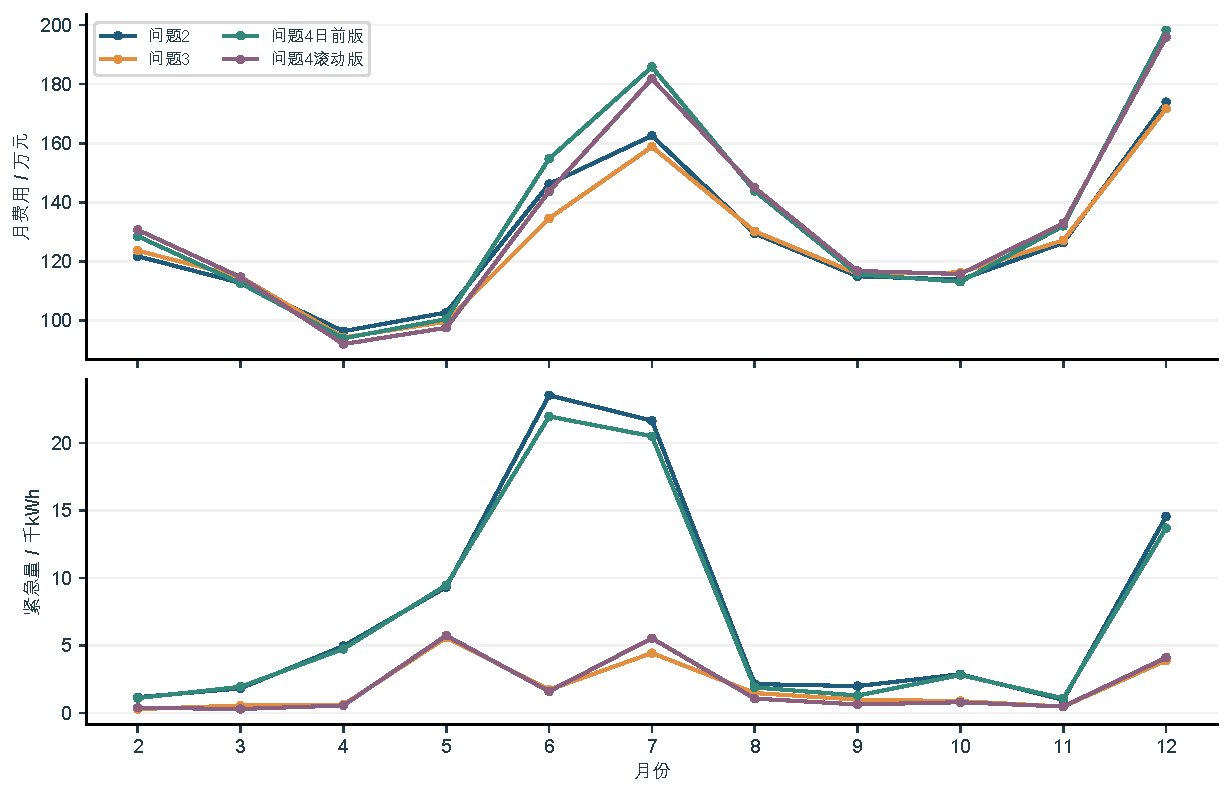
\includegraphics[width=0.95\linewidth]{figures/results/v2_monthly.pdf}
\caption{四组冻结主方案的月度实际费用与紧急购电量}\label{fig:v2-monthly}
\end{figure}
